\documentclass{article}

\usepackage[utf8]{inputenc}
\usepackage{listings}
\usepackage{microtype}
\usepackage[english,dutch]{babel}
\usepackage[a4paper]{geometry}
\usepackage{graphicx}

\frenchspacing
\parindent=0pt
\setlength{\textheight}{25.7cm}
\setlength{\textwidth}{16cm}
\topmargin 260mm \advance \topmargin -\textheight
\divide \topmargin by 2 \advance \topmargin -1in
\headheight 0pt \headsep 0pt \leftmargin 210mm \advance
\leftmargin -\textwidth
\divide \leftmargin by 2 \advance \leftmargin -1in
\oddsidemargin \leftmargin \evensidemargin \leftmargin


\lstset{language=Python, showstringspaces=false, basicstyle=\small,
  numbers=left, numberstyle=\tiny, numberfirstline=false, breaklines=true,
  stepnumber=1, tabsize=4, 
  commentstyle=\ttfamily, identifierstyle=\ttfamily,
  stringstyle=\itshape, }
\title{Billiards}
\author{Luuk - s2260018\\levi van Es - s2115409 }
\date{November 2018}

\begin{document}

\maketitle

\section{Introduction}
    Deze opdracht was nogal drastisch anders dan de voorgaande. 
    Het werd ons bij de eerste analyse van de opdracht al meteen duidelijk dat de
		opdracht de focus probeerde te leggen op het implementeren en gebruiken van classes. 
    Gelukkig hebben we beide al enige ervaring met class achtige elementen uit andere
		object georienteerde programmeertalen en was het concept voor ons niet vreemd. 
    Enige discussie was al duidleijk over onze gezamelijke aanpak van deze opdracht. 
    
\section{Code}
\subsection{Interface} 
De gebruikers interface waar de gebruiker als eerst mee geconfronteerd word moest
makkelijk en duidelijk in gebruik zijn met zo min mogelijk interactie en zo veel
mogelijk resultaat.
De wijze waarop dit moest gebeuren was zeer duidelijk gemaakt in de opdracht en
was daarom ook niet heel moeilijk om te implementeren.
Bij deze interface kwamen veel elementen terug uit vorige opdrachten en konden dus
simpel met elkaar geintegreerd worden en aangepast worden aan dit programma. 
\newline De automatische invoer is compleet gebouwd op de numpy functie np.loadtxt. 
Deze functie is perfect voor het omzetten van text in een array.
Wanneer dit is gebeurd is het maar een kwestie van de juiste waarde uit de array
op de goede plek in de 2 dementionale positie array te zetten en dat was het.
\subsection{Plotting}
\subsubsection{(v,t)plot}
Het v,t plot is misschien nog wel het meest invoudige gedeelte van dit project. 
Omdat de snelheidsvectors opgeslagen staan in een chronologische lijst is het heel
makkelijk om met pyplot gewoon de 1-dementionale snelheid van elke vector te plotten.
Dit was ook de laatste implementatie die wij hebben gemaakt aan het programma.
De werking van dit stukje werkt als volgt. De code vraagt aan de balclasses van
beide ballen de snelheid van de ballen op en plot deze snelheden in hun eigen
grafiek met as-opmaak.  
\subsubsection{Billiardplot}

\subsubsection{ASCII-Plot}
Het ASCII-Plot was bij de eerste gedachte een fluitje van een cent. 
Maar bij het verder lezen moest ook dit stuk van de code volgens een bepaalde
manier gecodeerd worden.
Hierbij moest een onbekende numpy functie gevonden worden die gebruikt moest
worden om de 2 dementionale array/lijst om te zetten naar een genormaliseerde versie hiervan.
Het vinden van deze functie bleek nog een groter opgeve dan gedacht.
Vandaar dat het even duurde voor deze was geimplementeerd. 
De algemene opstelling van het ASCII-plot is als volgt.
De posities van de ballen worden genormaliseerd en er word een 70 bij 18 zero array
aangemaakt waarin op de balcoordinaten het element word verhoogd met 1 of 2 afhankelijk van de bal.
In deze 2 dementionale array worden de elementen met 1 vervangen door een "o" en
worden de elementen met 2 vervangen door "x" en die met 3 worden vervangen door een plus.
Deze array word samengevoegd en alle 0 posities worden vervangen door een spatie.
Dit geeft resultaten zoals hieronder weergegeven.
Dit komt nauw overeen met de verwachtingsgrafiek daaronder. 


\begin{figure}
\begin{verbatim}
+----------------------------------------------------------------------+ 
|                                      o                               | 
|                                      o                               | 
|                                      o                               | 
|                                      o                               | 
|                                      o                               | 
|                                      o                               | 
|                                      o                               | 
|                                      o                               | 
|                                      o                               | 
|                                      o                               | 
|                                                                      | 
|                                                                      | 
|                                                                      | 
|                                                                      | 
|                                                                      | 
|                                                                      | 
|                                                                      | 
|                                                                      | 
+----------------------------------------------------------------------+ 
\end{verbatim}
\caption{Ascii-plot van voorbeelddata}
\label{fig:ascii-box}
\end{figure}
\begin{figure}
  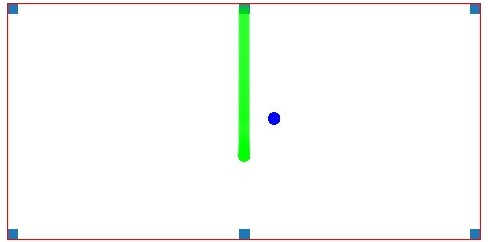
\includegraphics[width=\linewidth]{sampleplot.jpg}
  \caption{Correct referentieplot}
  \label{fig:exampleplot}
\end{figure}
\newpage

Zoals we kunnen zien komt de grafiek 1 op 1 overeen met de verwachtte grafiek.
Dit was voor ons een indicatie dat wij op het goede pad zaten en misschien nog maar
een paar kleine aanpassingen moesten maken. De problemen waar wij hier tegenaanliepen
waren voornamelijk de limitaties die ons werden opgelegd door de opdracht zelf.
Verder duurde het even voordat het plan van aanpak voor dit plot op was gesteld.
De realisatie van dit plan van aanpak bleek ook niet 1 op 1 vertaalbaar te zijn.
Als gevolg moest er een hoop aanpassingen gedaan worden om tot deze uitkomst te komen.  

\section{Tijdsverdeling}

\begin{tabular}{ l | p{6cm} p{6cm} }
   & Luuk & Levi \\
  \hline
  Week 1 & Begonnen aan de implementatie van de classes en de muurdetectie per bal 
  &  Begonnen aan de implementatie van de classes en de muurdetectie per bal \\
  Week 2 & Verdere optimalisatie muurdetectie en begin maken aan fysica implementatie voor de weerstand en verdere rolfysica 
  & -Begin maken aan user interface en zijn subsystemen(automatisch, handmatig) \\
  Week 3 & -Aestethica plot verbeteren en namaken na specificatie van de opdracht.
  \linebreak -Collisie detectie tussen n aantal ballen implementeren , testen en debuggen.
  & -Integratie invoersubsystemen in de userinterface en uitvoer formatting naar het juiste formaat voor de rest van de code  \\
  Week 4  & Samenvoegen van de interface, billiard en plot componenten in 1 uniforme functie.
  \linebreak Laatste testsituaties lopen \linebreak 
  - interface optimaliseren na specificaties & Ontwikkelen en implementeren van ASCII-grafiek.
  \linebreak - Verslag schrijven   \\
 
 
 
  
\end{tabular}

\section{Code}

 \begin{lstlisting}[frame=single, language=python]
 
 
 
 \end{lstlisting}

\end{document}
